\section{Radici di una equazione}

Data una funzione $f: [a,b] \subseteq \mathbb{R} \to \mathbb{R}$, vogliamo determinare un valore $x^* \in [a,b]$ tale che:
\[
f(x^*) = 0
\]
Diremo che $x^*$ è una \textbf{radice} (o uno \textbf{zero}) della funzione $f(x)$.

In generale, una radice $x^*$ può:
\begin{itemize}
    \item Esistere ed essere unica.
    \item Esistere ma non essere unica (es. $f(x) = \sin(x)$).
    \item Non esistere (es. $f(x) = e^x$).
\end{itemize}

I metodi che esamineremo, se la radice esiste, forniranno un'approssimazione di una di esse.  
Una caratteristica comune a tutti questi metodi è di essere di tipo \textbf{iterativo}:  
a partire da un'approssimazione iniziale $x_0$, viene prodotta una successione di approssimazioni $\{x_n\}_{n \ge 0}$ che, se il metodo è convergente, tende alla radice $x^*$:
\[
\lim_{n \to \infty} x_n = x^*
\]

\subsection{Il metodo di bisezione}
Il primo metodo che analizziamo è il metodo di bisezione.  
Si basa su due assunzioni fondamentali:
\begin{enumerate}
    \item La funzione $f(x)$ è \textbf{continua} in un intervallo chiuso e limitato $[a,b]$.
    \item Agli estremi dell'intervallo, la funzione assume valori di segno opposto, ovvero $f(a) \cdot f(b) < 0$.
\end{enumerate}

\begin{figure}[ht!]
    \centering
    \begin{tikzpicture}[scale=1.5]
        % Assi cartesiani
        \draw[->] (-0.5,0) -- (4,0) node[below] {$x$};
        \draw[->] (0,-1.5) -- (0,1.5) node[left] {$f(x)$};
        
        % Disegna la funzione
        \draw[thick, color=green!50!black] plot[smooth, domain=0.5:3.5] (\x, {cos(\x*60)+0.1*\x-0.5});
        
        % Punti e etichette
        \draw (1,0.05) -- (1,-0.05) node[below] {$a$};
        \draw (3,0.05) -- (3,-0.05) node[below] {$b$};
        \node[below, color=red] at (2.05, -0.05) {$x^*$};
        \fill[red] (2.05,0) circle (1.5pt);
        
        % Linee tratteggiate e valori
        \draw[dashed] (1,0) -- (1, {cos(60)+0.1*1-0.5});
        \draw[dashed] (0, {cos(60)+0.1*1-0.5}) -- (1, {cos(60)+0.1*1-0.5});
        \node[left] at (0, {cos(60)+0.1*1-0.5}) {$f(a) > 0$};
        
        \draw[dashed] (3,0) -- (3, {cos(180)+0.1*3-0.5});
        \draw[dashed] (0, {cos(180)+0.1*3-0.5}) -- (3, {cos(180)+0.1*3-0.5});
        \node[left] at (0, {cos(180)+0.1*3-0.5}) {$f(b) < 0$};
    \end{tikzpicture}
    \caption{Illustrazione del teorema degli zeri.}
    \label{fig:teorema_zeri}
\end{figure}

In base al \textbf{teorema degli zeri}, queste ipotesi garantiscono l'esistenza di almeno una radice $x^*$ nell'intervallo $(a,b)$.

Non sapendo dove si trovi $x^*$ all'interno di $[a,b]$, la migliore stima iniziale che possiamo fare è il punto medio dell'intervallo:
\[
x_1 = \frac{a+b}{2}
\]
A questo punto, si possono verificare tre casi:
\begin{enumerate}
    \item $f(x_1) = 0$: abbiamo trovato la radice.
    \item $f(a) \cdot f(x_1) < 0$: la radice si trova nell'intervallo $[a, x_1]$.
    \item $f(x_1) \cdot f(b) < 0$: la radice si trova nell'intervallo $[x_1, b]$.
\end{enumerate}
Ad ogni iterazione, l'ampiezza dell'intervallo di confidenza viene dimezzata.

\subsection{Implementazione e criteri di arresto}
Un'implementazione ``naive''\footnote{Per "implementazione naive" si intende una versione semplice e diretta dell'algoritmo che ignora problemi pratici di efficienza o stabilità numerica.} del metodo potrebbe essere:

\begin{lstlisting}
fa = f(a);
fb = f(b);
while true
    x1 = (a+b)/2;
    f1 = f(x1);
    if f1 == 0
        break;
    elseif fa*f1 < 0
        b = x1;
        fb = f1;
    else
        a = x1;
        fa = f1;
    end
end
\end{lstlisting}

Questo criterio di arresto non è robusto: a causa dell'aritmetica finita, la condizione `f1 == 0` potrebbe non verificarsi mai, anche se $x_1$ è molto vicino alla radice, portando a un ciclo infinito.

\paragraph{Esempio: Errore di valutazione}
Consideriamo il polinomio $p(x)=(x-1.1)^{20}(x-\pi)$, che ha una radice in $x=\pi$.  
Valutandolo in Matlab:
\begin{lstlisting}
p_coeffs = poly([1.1*ones(1,20), pi]);
polyval(p_coeffs, pi)
% ans = -5.5213e-05
\end{lstlisting}
Il risultato non è zero, e l'algoritmo naive andrebbe in loop.

\paragraph{Criterio basato sul numero di iterazioni}
Possiamo calcolare a priori il numero massimo di iterazioni necessarie per raggiungere una data tolleranza.  
Se $x_i$ è l'approssimazione al passo $i$, l'errore assoluto è maggiorato dalla semi-ampiezza dell'intervallo:
\[
|x^* - x_i| \le \frac{b_i - a_i}{2} = \frac{b-a}{2^i}
\]
Per garantire un'accuratezza `tol`, imponiamo:
\[
\frac{b-a}{2^i} \le \text{tol}
\quad \Rightarrow \quad
i \ge \log_2\!\left(\frac{b-a}{\text{tol}}\right)
\]
Il numero massimo di iterazioni sarà quindi:
\[
i_{\max} = \left\lceil \log_2\!\left(\frac{b-a}{\text{tol}}\right) \right\rceil
\]
\footnote{Questa formula calcola il numero massimo di iterazioni necessarie per garantire un errore inferiore a `tol`. L'operatore $\lceil \cdot \rceil$ (ceiling) arrotonda all'intero superiore.}

\begin{lstlisting}
fa = f(a);
fb = f(b);
imax = ceil(log2(b-a) - log2(tol));

for i = 1:imax
    x1 = (a+b)/2;
    f1 = f(x1);
    
    if f1 == 0
        break;
    elseif fa*f1 < 0
        b = x1;
        fb = f1;
    else
        a = x1;
        fa = f1;
    end
end
\end{lstlisting}

\paragraph{Criterio basato sul residuo (controllo efficace)}
Un criterio di arresto più efficiente si basa sulla "piccolezza" del valore della funzione, $|f(x)|$.  
Lo sviluppo di Taylor di $f(x)$ attorno alla radice $x^*$ è:
\[
f(x) = f(x^*) + f'(x^*)(x-x^*) + O(|x-x^*|^2)
\]
Dato che $f(x^*)=0$, otteniamo:
\[
|x-x^*| \approx \frac{|f(x)|}{|f'(x^*)|}
\]
e imponendo $|x-x^*| \le \text{tol}$, si ha:
\[
|f(x)| \le \text{tol} \cdot |f'(x^*)|
\]
Poiché $f'(x^*)$ non è noto, lo approssimiamo come:
\[
f'(x^*) \approx \frac{f(b_i)-f(a_i)}{b_i - a_i}
\]

\paragraph{Algoritmo di bisezione ottimizzato}
\begin{lstlisting}
% Versione ottimizzata del metodo di bisezione
fa = f(a);
fb = f(b);
imax = ceil(log2(b-a) - log2(tol));

for i = 1:imax
    x1 = (a+b)/2;
    f1 = f(x1);
    
    % Stima della derivata e criterio di arresto sul residuo
    df = abs(fb-fa)/(b-a);
    if abs(f1) <= tol*df
        break;
    end
    
    % Aggiornamento dell'intervallo
    if fa*f1 < 0
        b = x1; fb = f1;
    else
        a = x1; fa = f1;
    end
end
% x1 contiene la radice approssimata
\end{lstlisting}


\subsection{Ordine di Convergenza}
Abbiamo esaminato il metodo di bisezione, definito sotto le ipotesi $f \in C([a,b])$ e $f(a)f(b)<0$. L'errore $e_i = x^* - x_i$ al passo $i$ soddisfa:
$$ |e_i| \le \epsilon_i = \frac{b-a}{2^i} $$
con $\frac{\epsilon_{i+1}}{\epsilon_i} = \frac{1}{2}$, il che implica $\lim_{i \to \infty} \frac{\epsilon_{i+1}}{\epsilon_i} = \frac{1}{2}$.

\begin{definition}[Ordine di Convergenza]
Un generico metodo iterativo si dice \textbf{convergente} se $\lim_{i \to \infty} e_i = 0$.
Si dice che ha \textbf{ordine di convergenza $p$} se $p$ è il più grande numero reale positivo tale che esista una costante $C > 0$ (costante asintotica dell'errore) per cui:
$$ \lim_{i \to \infty} \frac{|e_{i+1}|}{|e_i|^p} = C < \infty $$
\end{definition}

Per $i$ sufficientemente grande, vale $|e_{i+1}| \approx C |e_i|^p$.
\begin{itemize}
    \item Affinché ci sia convergenza, deve aversi $p \ge 1$.
    \item Se $p=1$, la convergenza è \textbf{lineare}. In questo caso, per $i$ grande, abbiamo:
          \begin{align*}
              |e_{i+1}| &\approx C |e_i| \\
              |e_{i+2}| &\approx C |e_{i+1}| \approx C^2 |e_i| \\
              &\vdots \\
              |e_{i+k}| &\approx C^k |e_i| 
          \end{align*}
          Questa successione tende a zero per $k \to \infty$ se e solo se $C < 1$. Pertanto, un metodo di ordine 1 è convergente se e solo se la sua costante asintotica dell'errore è minore di 1.
    \item Se $p=2$, la convergenza è \textbf{quadratica}.
    
\end{itemize}

\begin{osservazione}
Il metodo di bisezione, se applicabile, è sempre convergente, ha ordine $p=1$ e costante asintotica $C=1/2$.
\end{osservazione}

Un ordine $p$ più elevato implica una convergenza più rapida. Confrontiamo due metodi con $C=0.1$ e $|e_0|=0.1$:

\begin{table}[ht!]
\centering
\caption{Confronto tra convergenza lineare e quadratica ($|e_{i+1}| \approx C|e_i|^p$)}
\begin{tabular}{ccc}
\toprule
$i$ & Errore ($p=1$) & Errore ($p=2$) \\
\midrule
0 & $10^{-1}$ & $10^{-1}$ \\
1 & $10^{-2}$ & $10^{-3}$ \\
2 & $10^{-3}$ & $10^{-7}$ \\
3 & $10^{-4}$ & $10^{-15}$ \\
\bottomrule
\end{tabular}
\end{table}
È evidente che è bene ricercare metodi di ordine più elevato.

\paragraph{Condizionamento del Problema}
Vogliamo determinare $x^*$ tale che $f(x^*) = 0$. Se invece abbiamo una soluzione perturbata $\tilde{x}$ tale che $f(\tilde{x}) \neq 0$, studiamo come la perturbazione sul valore $f(\tilde{x})$ influenza l'errore $|\tilde{x} - x^*|$.
Usando Taylor: $f(\tilde{x}) \approx f'(x^*)(\tilde{x} - x^*)$, da cui:
$$ |\tilde{x} - x^*| \approx \frac{|f(\tilde{x})|}{|f'(x^*)|} $$
Il fattore $K = \frac{1}{|f'(x^*)|}$ è il \textbf{numero di condizione} del problema.
\begin{itemize}
    \item Se $|f'(x^*)| \ >> 1$ (non vicino a zero), il problema è \textbf{ben condizionato}.
    \item Se $|f'(x^*)| \approx 0$, il problema è \textbf{mal condizionato}.
\end{itemize}

\begin{definition}[Molteplicità di una radice]
Una radice $x^*$ ha \textbf{molteplicità $m \ge 1$} se $f(x^*) = f'(x^*) = \dots = f^{(m-1)}(x^*) = 0$ e $f^{(m)}(x^*) \neq 0$.
Se $m=1$, la radice è \textbf{semplice}. Se $m>1$, la radice è \textbf{multipla}.
\end{definition}

\begin{osservazione}
L'approssimazione di una radice multipla dà origine ad un problema \textbf{sempre mal condizionato}.
\end{osservazione}

\subsection{Metodo di Newton}
Il metodo di Newton è un metodo iterativo che, a partire da un'approssimazione $x_0$, costruisce la successione $\{x_i\}$ utilizzando l'interpretazione geometrica della derivata.

L'equazione della retta tangente al grafico di $f(x)$ nel punto $(x_0, f(x_0))$ è data da $y - f(x_0) = f'(x_0)(x - x_0)$. La nuova approssimazione $x_1$ si trova intersecando questa retta con l'asse delle $x$ (retta di equazione $y=0$). Dobbiamo quindi risolvere il sistema:
\[
\begin{cases} 
y - f(x_0) = f'(x_0)(x - x_0) & \leftarrow \text{retta tangente} \\
y = 0 & \leftarrow \text{asse x}
\end{cases}
\]
Sostituendo $y=0$ nella prima equazione e chiamando la soluzione $x_1$, otteniamo:
$$ -f(x_0) = f'(x_0)(x_1 - x_0) $$
Da cui si ricava la nuova approssimazione:
$$ x_1 = x_0 - \frac{f(x_0)}{f'(x_0)} $$
In generale, iterando questo procedimento, si ottiene la formula del metodo di Newton:
$$ x_{i+1} = x_i - \frac{f(x_i)}{f'(x_i)}, \quad i=0, 1, \dots $$

% --- INSERISCI QUI IL GRAFICO ---
\begin{figure}[ht!] % Ho cambiato [h!] in [ht!] come suggerito dal warning
\centering
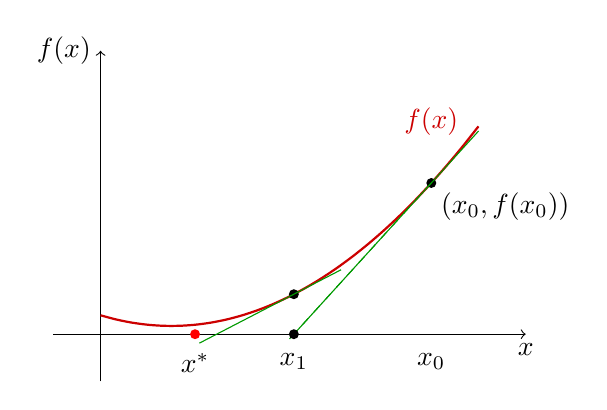
\begin{tikzpicture}[scale=1.2]
    % Assi
    \draw[->] (-0.5,0) -- (4.5,0) node[below] {$x$};
    \draw[->] (0,-0.5) -- (0,3) node[left] {$f(x)$};
    
    % Curva f(x)
    \draw[thick, color=red!80!black] plot[smooth, domain=0:4] (\x, {0.2*(\x-1)^2 + 0.1*\x});
    \node[above, color=red!80!black] at (3.5, 2) {$f(x)$};
    
    % Punto x0 e tangente
    \coordinate (x0) at (3.5, {0.2*(3.5-1)^2 + 0.1*3.5});
    \fill (x0) circle (1.5pt);
    \node[below right] at (x0) {$(x_0, f(x_0))$};
    \draw (3.5,-0.1) node[below] {$x_0$};
    
    % Calcolo della derivata in x0 (pendenza)
    % f'(x) = 0.4*(x-1) + 0.1 -> f'(3.5) = 0.4*2.5 + 0.1 = 1.1
    % Retta: y - f(x0) = 1.1 * (x - x0)
    \draw[color=green!60!black] (x0) -- +(-1.5, -1.5*1.1) coordinate (endtan0); % Disegna un pezzo della tangente
    \draw[color=green!60!black] (x0) -- +(0.5, 0.5*1.1); % Altro pezzo
    
    % Intersezione x1
    % y=0 => -f(x0) = 1.1 * (x1 - x0) => x1 = x0 - f(x0)/1.1
    % f(3.5) = 0.2*2.5^2 + 0.1*3.5 = 0.2*6.25 + 0.35 = 1.25 + 0.35 = 1.6
    % x1 = 3.5 - 1.6/1.1 = 3.5 - 1.4545... = 2.045...
    \coordinate (x1_inter) at (3.5 - 1.6/1.1, 0);
    \draw[dashed, color=green!60!black] (x0) -- (x1_inter);
    \draw (x1_inter)+(0,-0.1) node[below] {$x_1$};
    \fill (x1_inter) circle (1.5pt);

    % Punto x1 sulla curva e tangente
    \coordinate (x1) at (3.5 - 1.6/1.1, {0.2*((3.5 - 1.6/1.1)-1)^2 + 0.1*(3.5 - 1.6/1.1)});
    \fill (x1) circle (1.5pt);
    % f'(x1) = 0.4*(x1-1) + 0.1 = 0.4*(1.045...) + 0.1 = 0.418 + 0.1 = 0.518
    \draw[color=green!60!black] (x1) -- +(-1.0, -1.0*0.518);
    \draw[color=green!60!black] (x1) -- +(0.5, 0.5*0.518);
    
    % Intersezione x* (radice) - approssimata
    \coordinate (x_star) at (1,0); % f(1)=0.1, ma facciamo finta che sia la radice per semplicità
    \draw (x_star)+(0,-0.1) node[below] {$x^*$};
    \fill[red] (x_star) circle (1.5pt);

\end{tikzpicture}
\caption{Interpretazione geometrica del metodo di Newton.}
\label{fig:newton}
\end{figure}
% --- FINE GRAFICO ---

\paragraph{Considerazioni sul Metodo di Newton}
\begin{enumerate}
    \item È richiesta la derivabilità di $f(x)$ (almeno $f \in C^2$ in un intorno della radice per l'analisi).
    \item Il costo per iterazione è 1 valutazione di $f(x)$ e 1 valutazione di $f'(x)$.
\end{enumerate}

\begin{teorema}[Convergenza di Newton]
    Sia $f(x) \in C^{(2)}$ in un intorno della radice $x^*$. Supponiamo che il metodo di Newton converga a $x^*$, e che $x^*$ sia semplice. Allora l'ordine di convergenza è (almeno) 2.
\end{teorema}
\begin{proof}[Dimostrazione (schizzo)]
Sviluppando $f(x^*)$ in Taylor attorno a $x_i$:
$$ 0 = f(x^*) = f(x_i) + f'(x_i)(x^* - x_i) + \frac{1}{2} f''(\xi_i)(x^* - x_i)^2, \quad \xi_i \in (x_i, x^*) $$
Ponendo $e_i = x^* - x_i$ e $e_{i+1} = x^* - x_{i+1}$:
$$ 0 = f(x_i) + f'(x_i)e_i + \frac{1}{2} f''(\xi_i)e_i^2 $$
Dividendo per $f'(x_i)$ e usando $x_{i+1} = x_i - f(x_i)/f'(x_i)$:
$$ 0 = -(x_{i+1} - x_i) + e_i + \frac{1}{2} \frac{f''(\xi_i)}{f'(x_i)} e_i^2 $$
$$ 0 = -(x_{i+1} - x_i) + (x^* - x_i) + \frac{1}{2} \frac{f''(\xi_i)}{f'(x_i)} e_i^2 = (x^* - x_{i+1}) + \frac{1}{2} \frac{f''(\xi_i)}{f'(x_i)} e_i^2 $$
$$ e_{i+1} = - \frac{1}{2} \frac{f''(\xi_i)}{f'(x_i)} e_i^2 $$
Passando al limite per $i \to \infty$:
$$ \lim_{i \to \infty} \frac{|e_{i+1}|}{|e_i|^2} =  \frac{1}{2} \left|\frac{f''(x^*)}{f'(x^*)} \right| = C $$
Questo dimostra la convergenza quadratica ($p=2$).
\end{proof}

\begin{osservazione}[Radici multiple]
    Nel caso di una radice multipla, con molteplicità $m > 1$, si può dimostrare che:
    $$ \lim_{i \to \infty} \frac{|e_{i+1}|}{|e_i|} = \frac{m-1}{m} $$
    ovvero, l'ordine di convergenza del metodo di Newton diventa lineare ($p=1$), come conseguenza del mal condizionamento del problema.
    \end{osservazione}